\begin{figure*}[p]
  \centering
\subfloat[\BPNoise~bootstrapped distributions and ranks given by NPSK.]{
  \begin{minipage}{\textwidth}
    \begin{minipage}[t]{0.03\textwidth}
      \footnotesize\raggedleft
      \vspace{0.65cm}
      SIMSE\\[0.6cm]
      L1\\[0.65cm]
      JTFS\\[0.65cm]
      DTW
    \end{minipage}%
    \hspace{0.01\textwidth}%
    \begin{minipage}[t]{0.96\textwidth}
      \centering
      \begin{minipage}[t]{0.31\textwidth}
        \centering
        \normalsize\bfseries MSS\\[0.3em]
        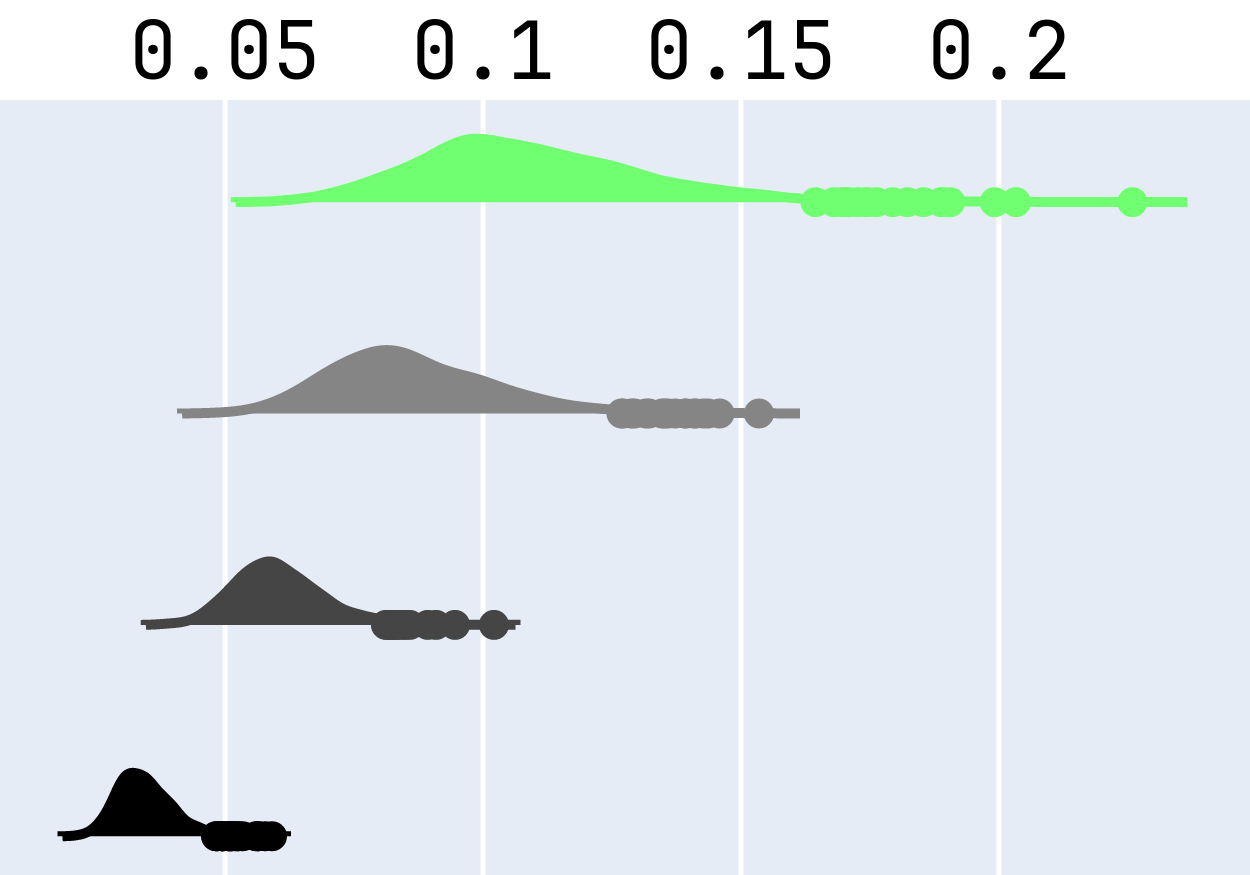
\includegraphics[width=\linewidth]{images/npsk_MSS_0.png}
      \end{minipage}
      \hspace{0.015\textwidth}%
      \begin{minipage}[t]{0.31\textwidth}
        \centering
        \normalsize\bfseries P-Loss\\[0.3em]
        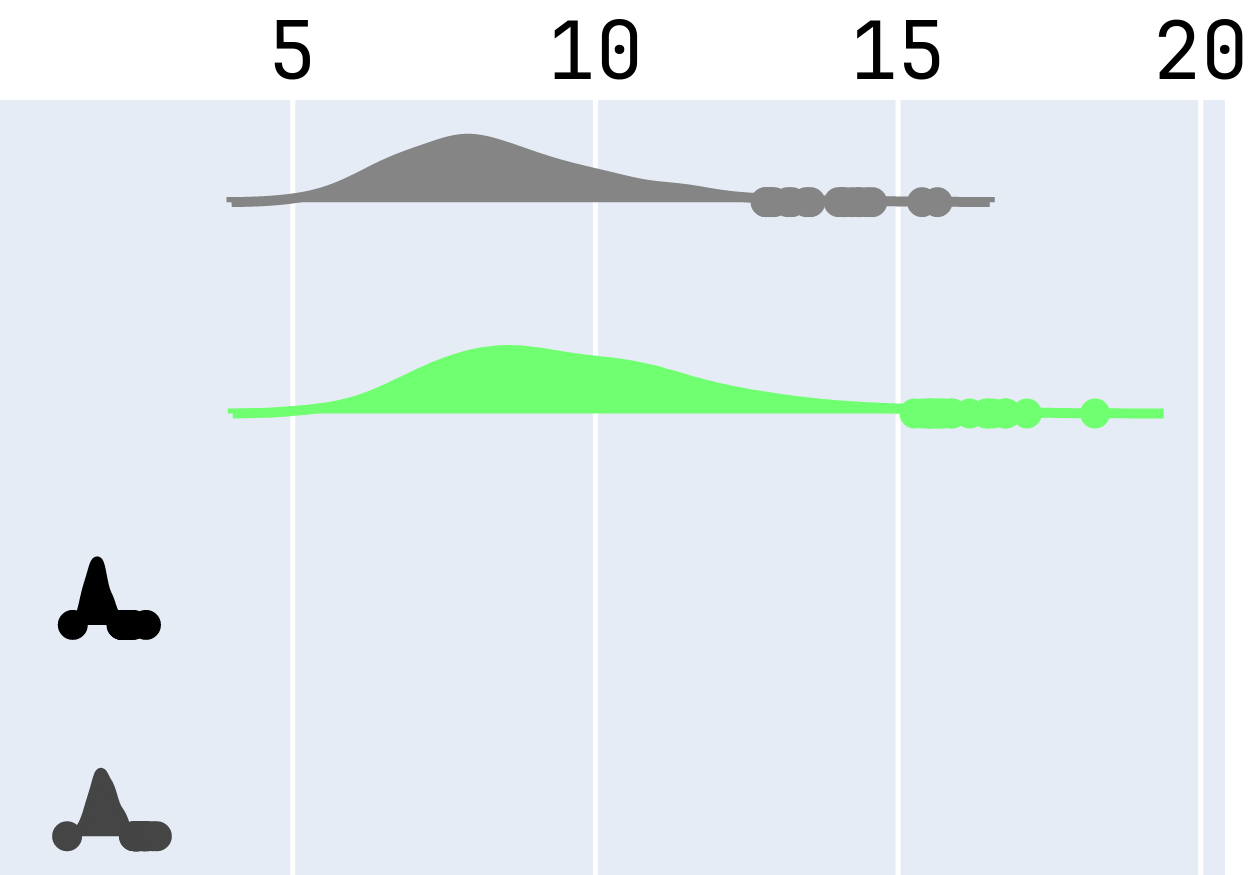
\includegraphics[width=\linewidth]{images/npsk_P-Loss_0.png}
      \end{minipage}
      \hspace{0.01\textwidth}%
      \begin{minipage}[t]{0.31\textwidth}
        \centering
        \normalsize\bfseries Likert\\[0.3em]
        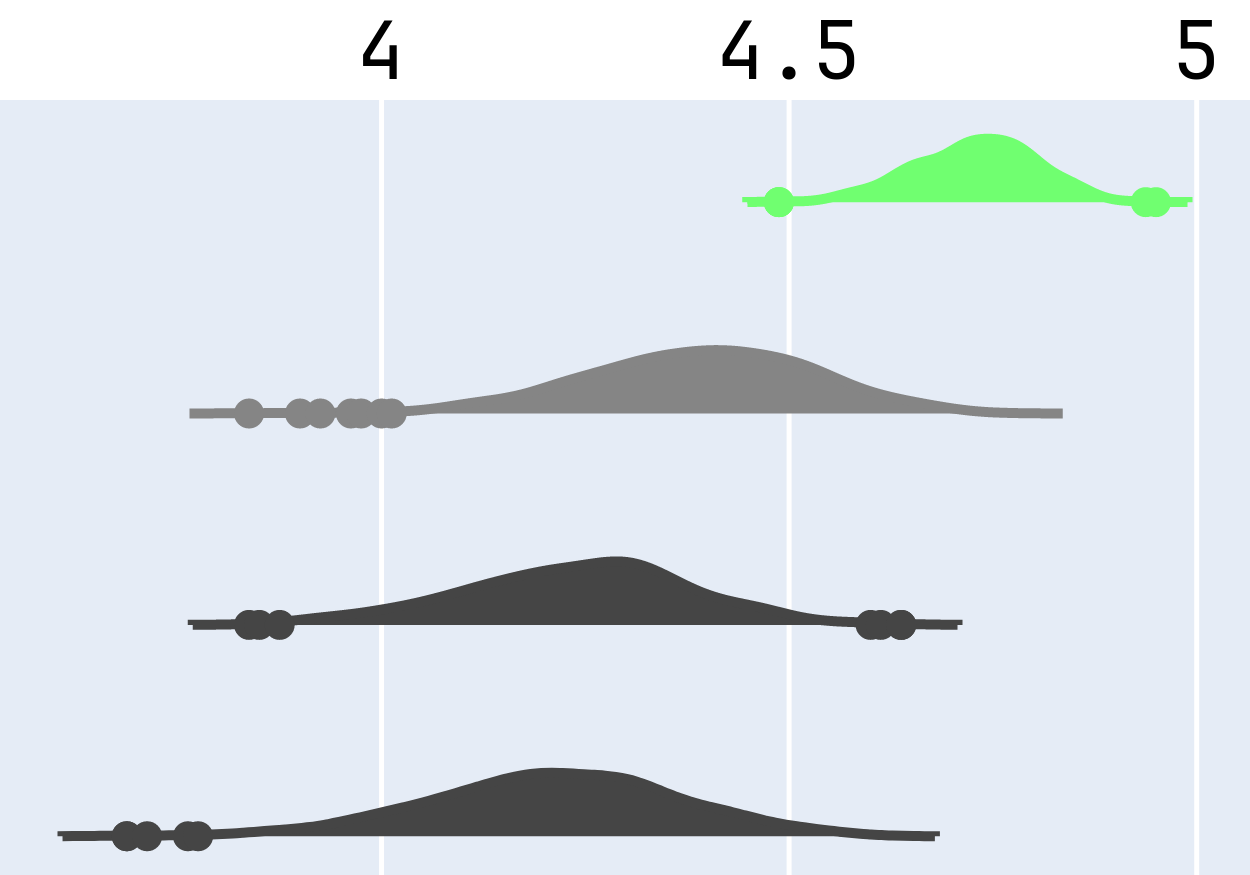
\includegraphics[width=\linewidth]{images/npsk_likert_0.png}
      \end{minipage}
    \end{minipage}
  \end{minipage}
  \label{fig:npsk_p0}
}\\[0.5em]

% 2nd row
\subfloat[\AddSineSaw~bootstrapped distributions and ranks given by NPSK.]{
  \begin{minipage}{\textwidth}
    \begin{minipage}{0.03\textwidth}
      \footnotesize\raggedleft
      \vspace{0.5cm}
      SIMSE\\[0.6cm]
      L1\\[0.65cm]
      JTFS\\[0.65cm]
      DTW
    \end{minipage}%
    \begin{minipage}{0.98\textwidth}\centering
      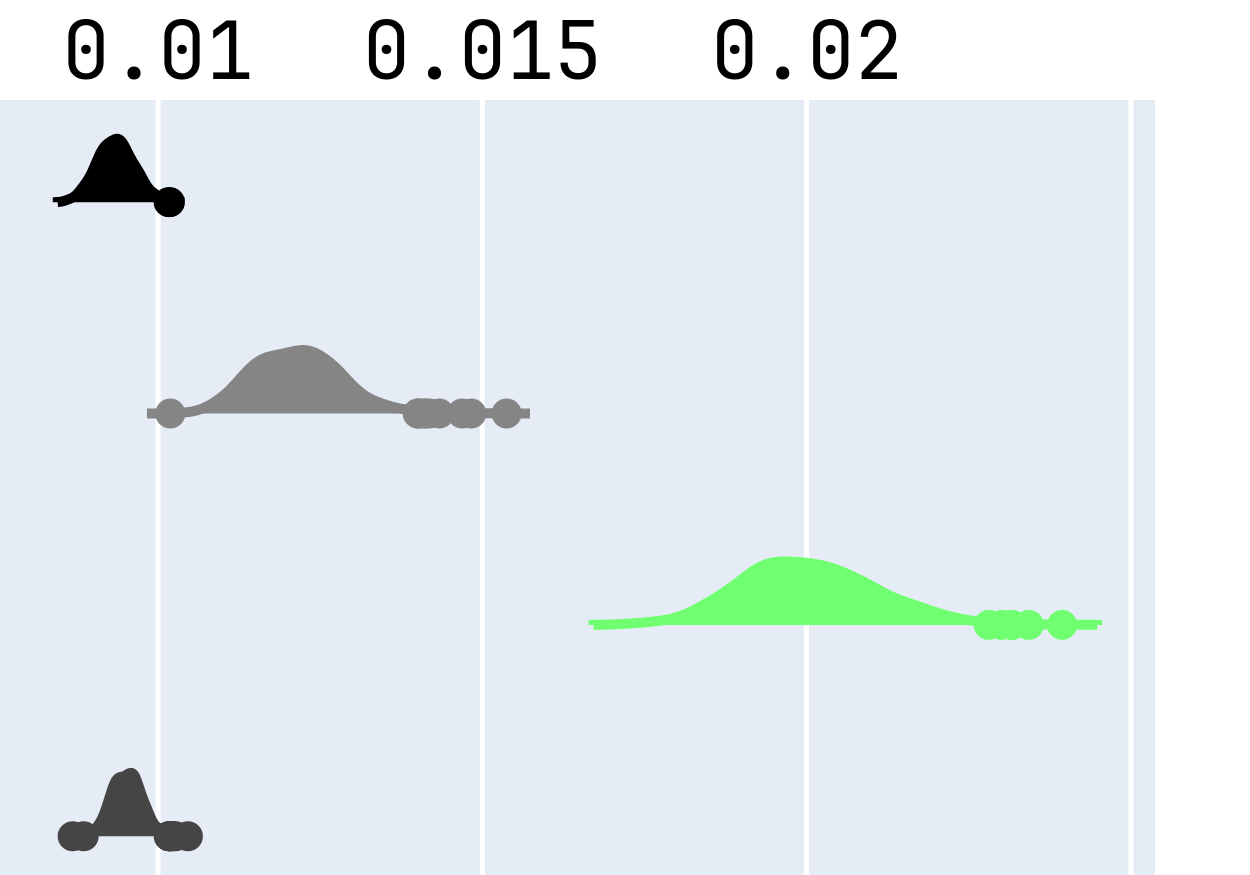
\includegraphics[width=0.31\textwidth]{images/npsk_MSS_1.png}%
      \hspace{0.015\textwidth}%
      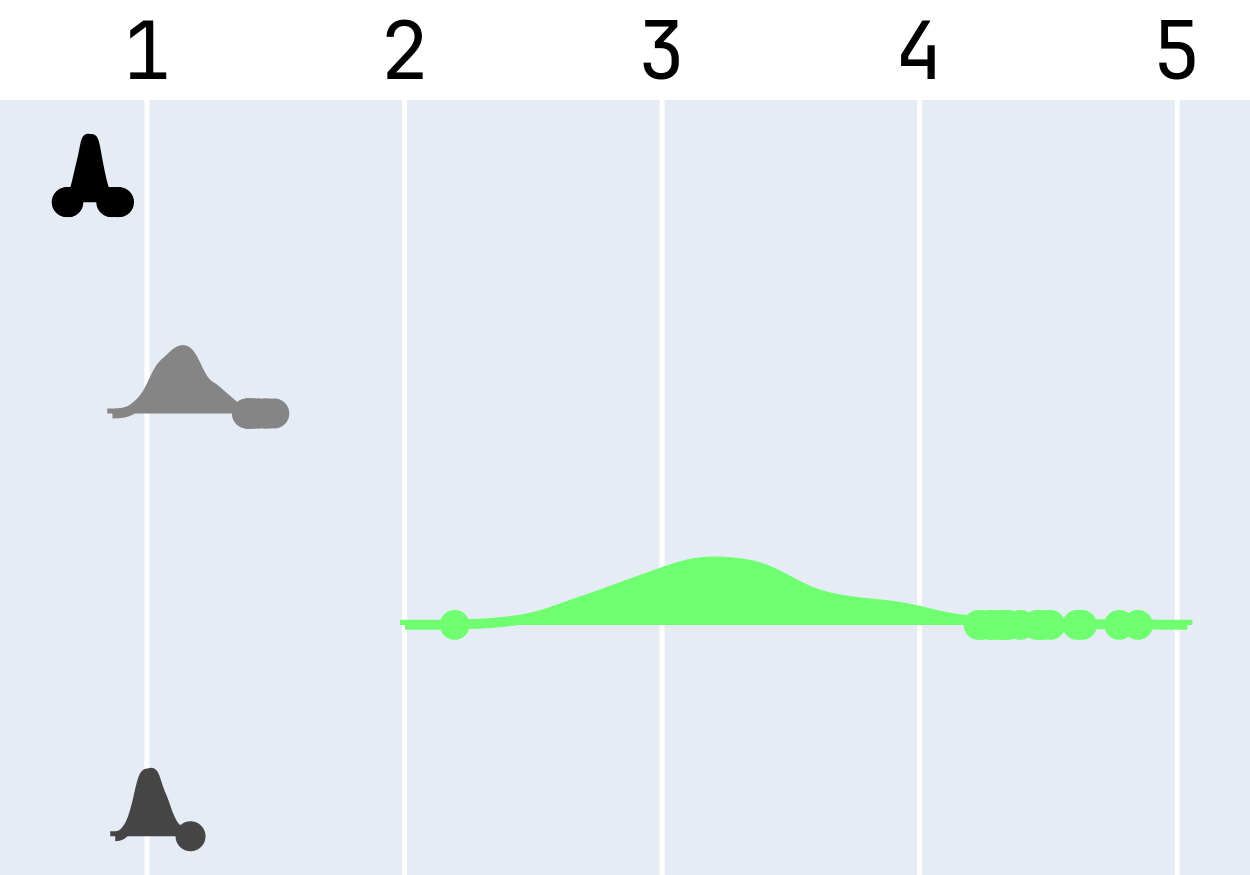
\includegraphics[width=0.31\textwidth]{images/npsk_P-Loss_1.png}%
      \hspace{0.015\textwidth}%
      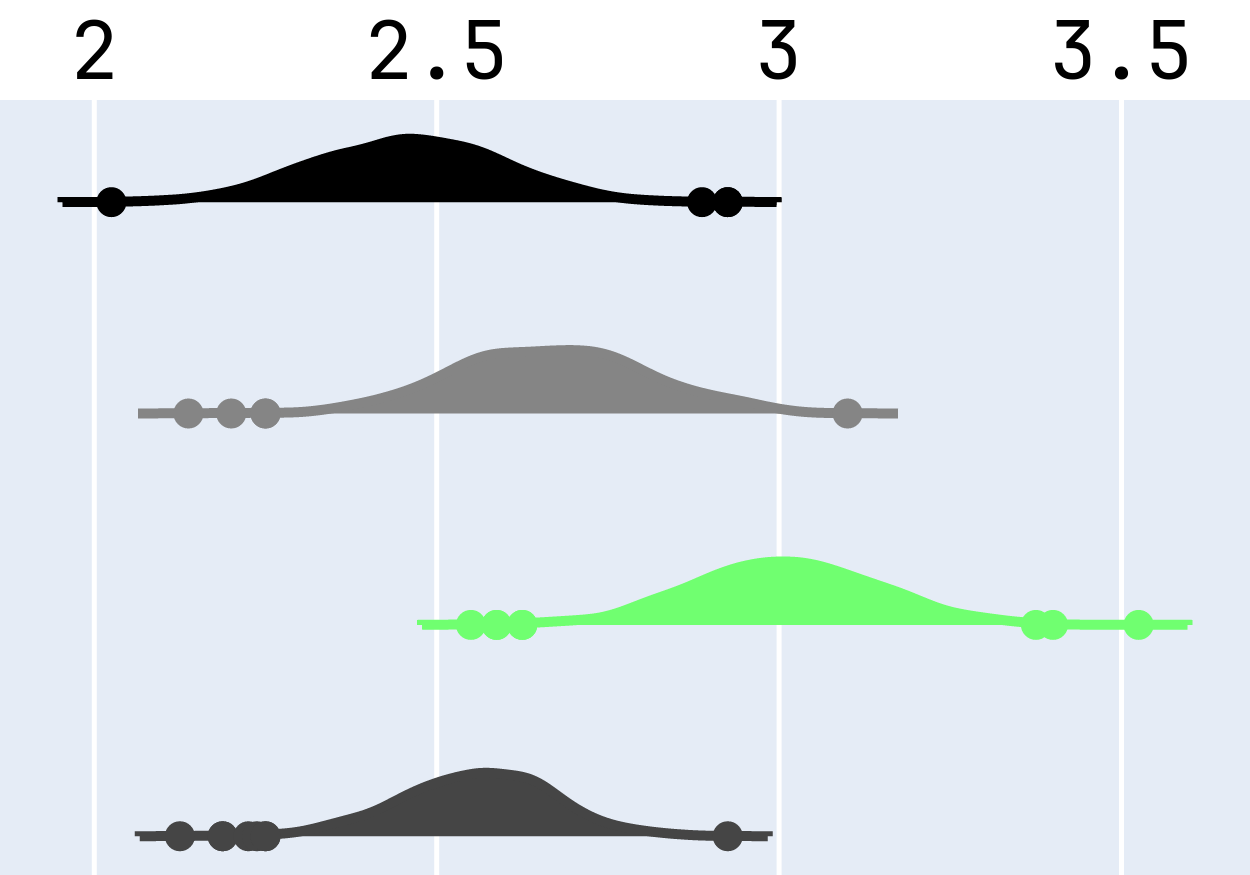
\includegraphics[width=0.31\textwidth]{images/npsk_likert_1.png}
    \end{minipage}
  \end{minipage}
  \label{fig:npsk_p1}
}\\[0.5em]

% 3rd row
\subfloat[\AmpMod~bootstrapped distributions and ranks given by NPSK.]{
  \begin{minipage}{\textwidth}
    \begin{minipage}{0.03\textwidth}
      \footnotesize\raggedleft
      \vspace{0.5cm}
      SIMSE\\[0.6cm]
      L1\\[0.65cm]
      JTFS\\[0.65cm]
      DTW
    \end{minipage}%
    \begin{minipage}{0.98\textwidth}\centering
      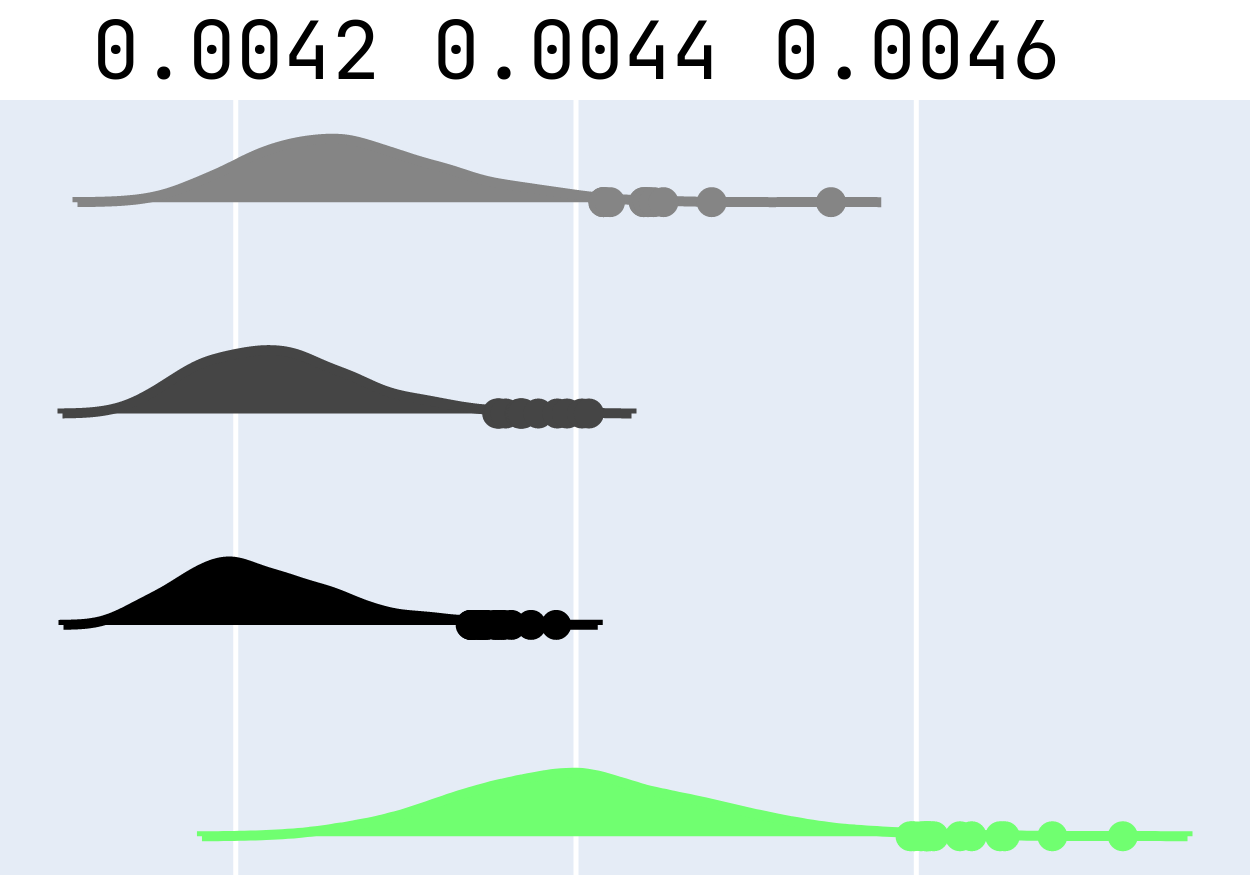
\includegraphics[width=0.31\textwidth]{images/npsk_MSS_2.png}%
      \hspace{0.015\textwidth}%
      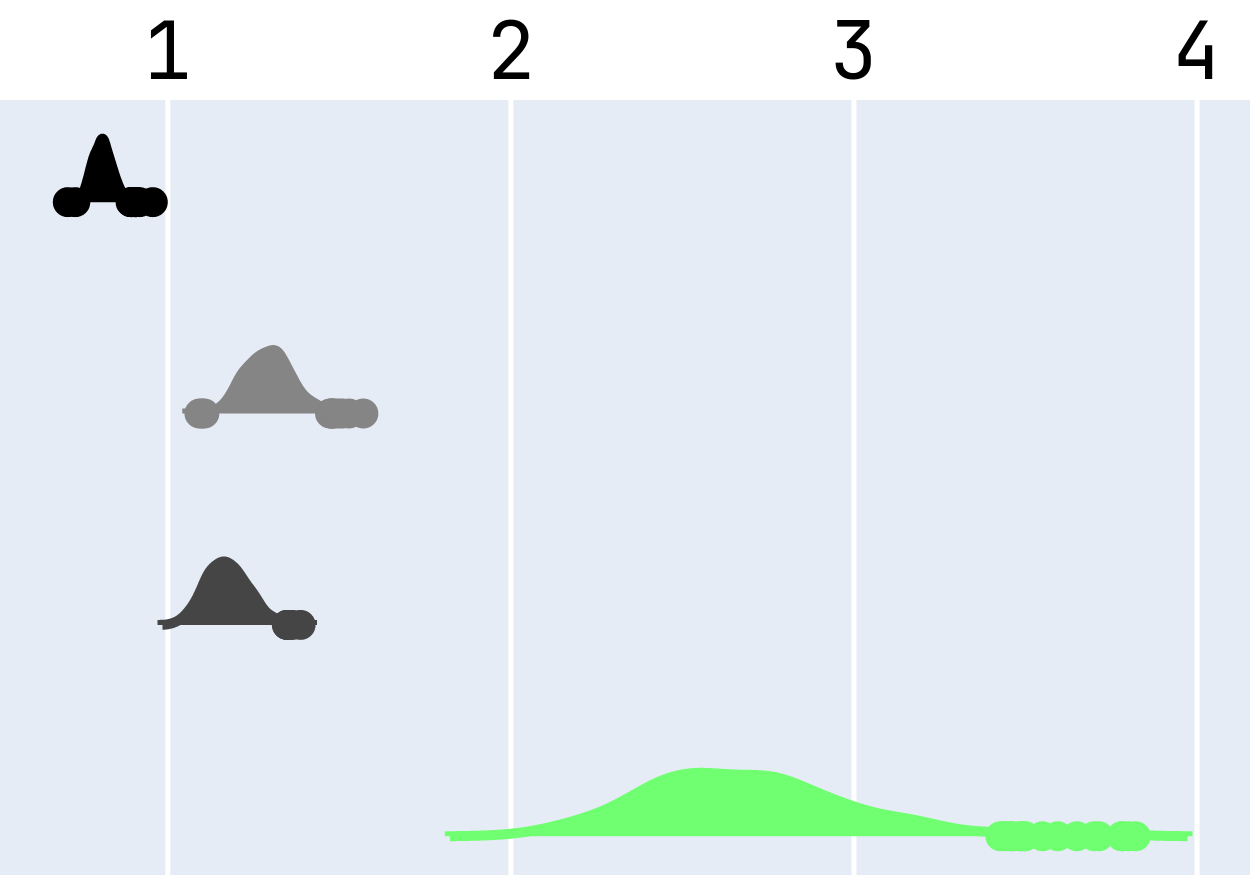
\includegraphics[width=0.31\textwidth]{images/npsk_P-Loss_2.png}%
      \hspace{0.015\textwidth}%
      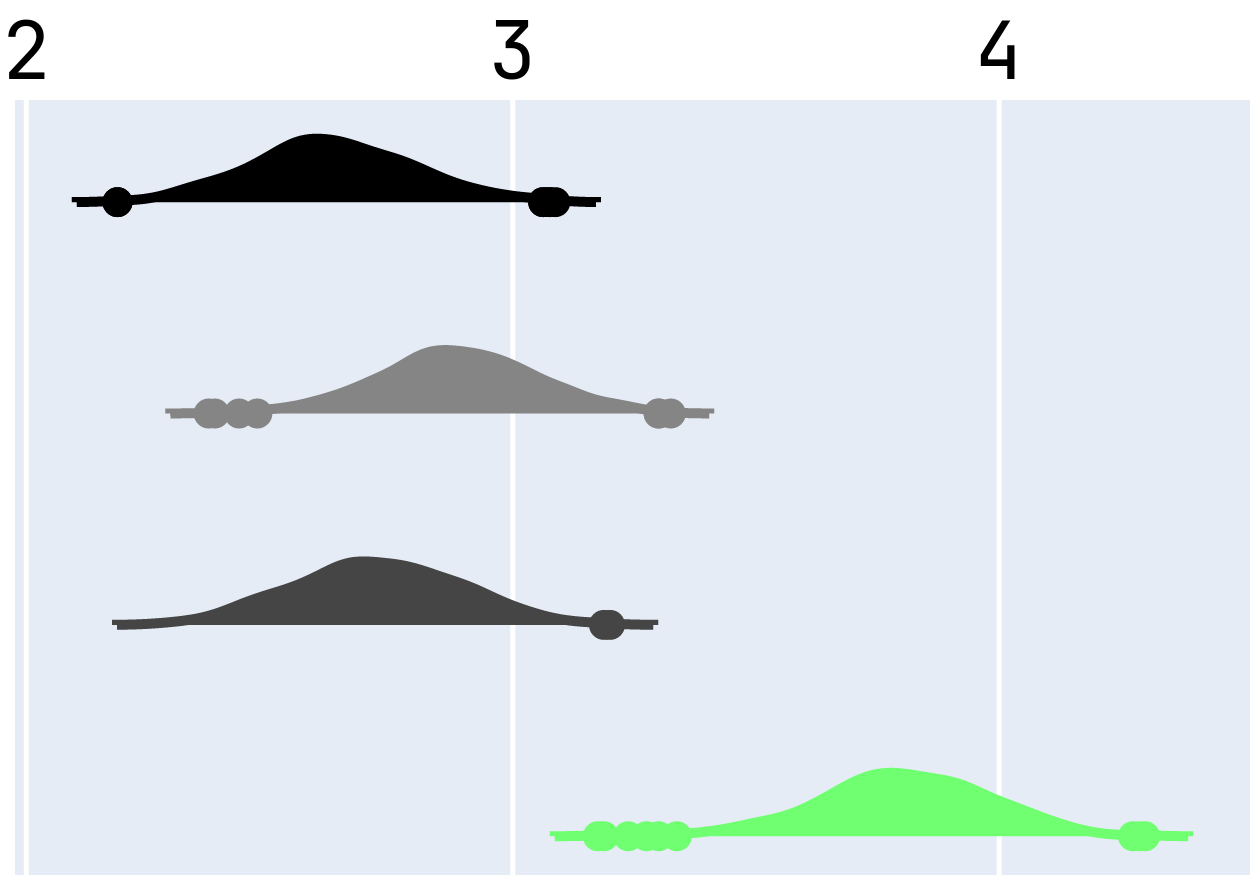
\includegraphics[width=0.31\textwidth]{images/npsk_likert_2.png}
    \end{minipage}
  \end{minipage}
  \label{fig:npsk_p2}
}\\[0.5em]

% 4th row
\subfloat[\FMMod~bootstrapped distributions and ranks given by NPSK.]{
  \begin{minipage}{\textwidth}
    \begin{minipage}{0.03\textwidth}
      \footnotesize\raggedleft
      \vspace{0.5cm}
      SIMSE\\[0.6cm]
      L1\\[0.65cm]
      JTFS\\[0.65cm]
      DTW
    \end{minipage}%
    \begin{minipage}{0.98\textwidth}\centering
      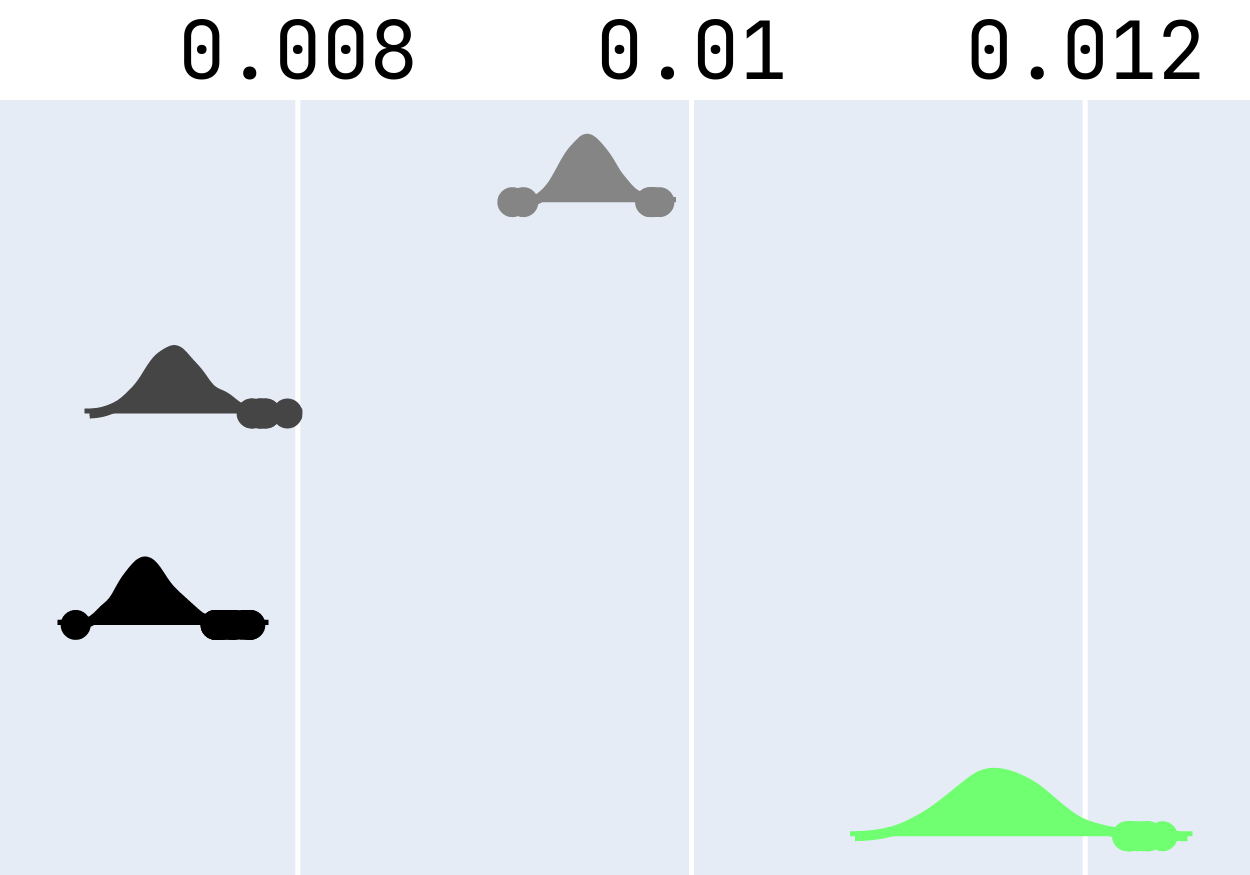
\includegraphics[width=0.31\textwidth]{images/npsk_MSS_3.png}%
      \hspace{0.015\textwidth}%
      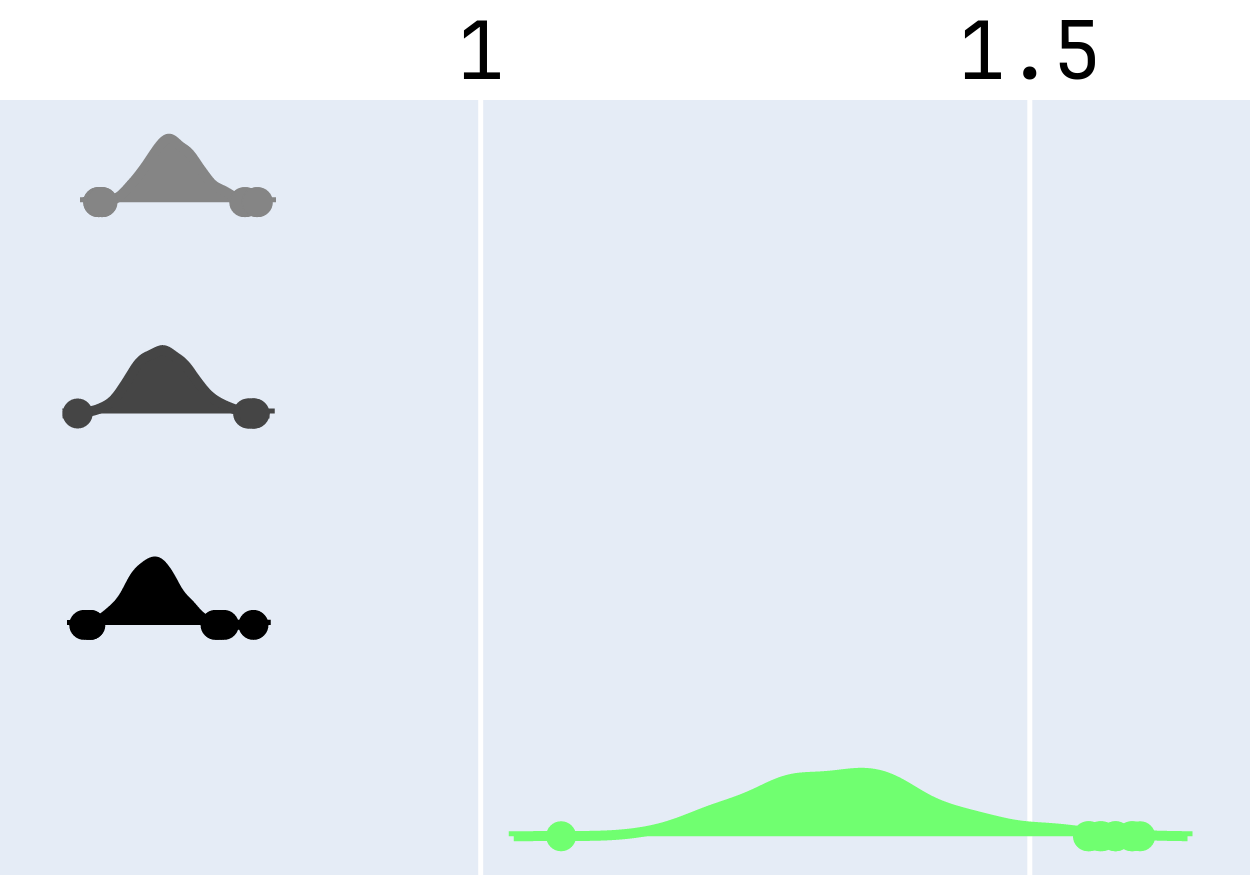
\includegraphics[width=0.31\textwidth]{images/npsk_P-Loss_3.png}%
      \hspace{0.015\textwidth}%
      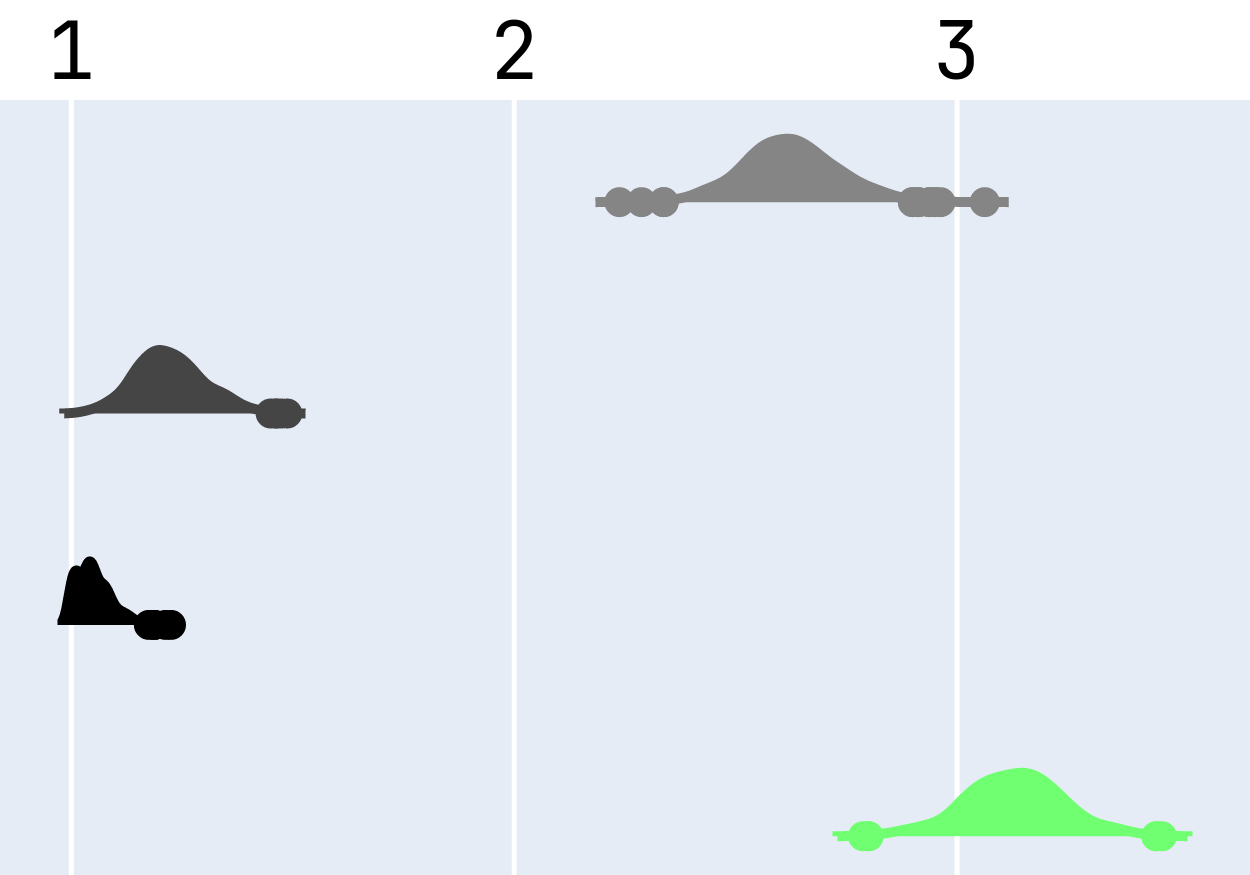
\includegraphics[width=0.31\textwidth]{images/npsk_likert_3.png}
    \end{minipage}
  \end{minipage}
  \label{fig:npsk_p3}
}

\caption{Distributions and ranks of the loss functions based on three different performance measures. From left to right, the performance measures are: MSS, P-Loss, and Likert. Higher values indicate better performance. Rank colors are \colorbox{rank1}{\textcolor{black}{\textbf{1}}} \colorbox{rank2}{\textcolor{white}{\textbf{2}}} \colorbox{rank3}{\textcolor{white}{\textbf{3}}} \colorbox{rank4}{\textcolor{white}{\textbf{4}}}.}
\label{fig:npsk_all}
\end{figure*}
